\pdfoutput=1 
\documentclass[12pt,a4paper]{article}
\usepackage{cite}
\usepackage{xcolor}
\definecolor{darkPurple}{HTML}{3333B2}
\definecolor{forestGreen}{HTML}{337700}
\definecolor{shadecolor}{HTML}{CCCCCC}
\definecolor{darkGrey}{HTML}{4E4F86}
\definecolor{Crimson}{HTML}{DC143C}
\definecolor{transparentBlue}{HTML}{EBEBF8}
\usepackage{hyperref}
\hypersetup{colorlinks=true, linkcolor=darkPurple, citecolor=darkPurple}
\usepackage[pdftex]{graphicx}
\graphicspath{{./figures/}}
\usepackage[cmex10]{amsmath}
\usepackage{amssymb}
\usepackage{multirow}	
\usepackage[]{subfig}
\usepackage[toc]{appendix}
\usepackage{listings}
\hypersetup{
    bookmarks=true,         % show bookmarks bar?
    unicode=false,          % non-Latin characters in Acrobat’s bookmarks
    pdftoolbar=true,        % show Acrobat’s toolbar?
    pdfmenubar=true,        % show Acrobat’s menu?
    pdffitwindow=false,     % window fit to page when opened
    pdfstartview={FitH},    % fits the width of the page to the window
    pdftitle={My title},    % title
    pdfauthor={Author},     % author
    pdfsubject={Subject},   % subject of the document
    pdfcreator={Creator},   % creator of the document
    pdfproducer={Producer}, % producer of the document
    pdfkeywords={keyword1, key2, key3}, % list of keywords
    pdfnewwindow=true,      % links in new PDF window
    colorlinks=true,       % false: boxed links; true: colored links
    linkcolor=blue,          % color of internal links (change box color with linkbordercolor)
    citecolor=green,        % color of links to bibliography
    filecolor=magenta,      % color of file links
    urlcolor=cyan           % color of external links
}
\usepackage[english]{babel}
\lstset { %
  language=C,
  backgroundcolor=\color{black!5}, % set backgroundcolor
  basicstyle=\footnotesize,        % the size of the fonts that are used for the code
  commentstyle=\color{forestGreen},    % comment style
  keywordstyle=\color{blue},       % keyword style
  keepspaces=true,                 % keeps spaces in text, useful for keeping indentation of code (possibly needs columns=flexible)
  showspaces=false,
  showstringspaces=false
}
% Font settings to get IEEE-style fonts
\renewcommand{\sfdefault}{phv}
\renewcommand{\rmdefault}{ptm}
\renewcommand{\ttdefault}{pcr}
\newcommand{\tab}[0]{\hspace{.2\textwidth}}
\newcommand{\tabone}[0]{\hspace{1em}}
\newcommand{\tabtwo}[0]{\hspace{2em}}
\title{Ajit Serial Driver Documentation}
\author{Harshal Kalyane }

\date{\today}
\begin{document}
\maketitle

\newpage
\tableofcontents
\newpage

\section{Introduction}
\tabtwo Driver is software which is used to do hardware specific operation, and create abstraction between OS and Hardware.\\
There are mainly three types of driver in Linux: \\
 1)Network Driver \\ 2) Block Driver\\ 3) Char driver\\
Network driver deals with networks packets and  network hardware. Block driver deals with storage devices and file system. Char driver is mainly used for those devices which are not part of the above two categories.

\section{Char driver} 
\tabtwo As name suggests, these types of drivers communicate with hardware by character (byte). Protocol  of communication is device dependant. Serial char driver can be developed from scratch or from already built char driver. To reduce complexity and  developing time Linux mainline kernel has tty driver. TTY driver gives standard abstract layer between OS and low level serial driver.

TTY core and TTY line discipline is provided by kernel itself. Developer needs to design only low level serial driver. Low level level driver has to do only hardware specific operation and need to fill data in TTY core data structure. Low level serial does not need to worry about user space interaction, it is handles by TTY core. 
	\begin{figure}[h!]
	\centering
	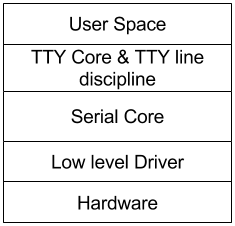
\includegraphics[width=0.5\textwidth]{./figs/Serial_Driver_block.png}
	\caption{Block Diagram of Serial Driver}
	\label{fig1}
	\end{figure}
Every driver has to do following things:
\\1)\_\_init  \textless function\_name\textgreater :
This get loaded on serial driver initialization. It registers itself and respective port in kernel for it’s hardware.
\\2) \_\_exit \textless function\_name\textgreater : This get called at time unloading of module or driver.
\\
\section{AJIT Serial Driver}
This driver is written for Ajit serial device.\\
\textbf{int \_\_init Ajit\_init(void)} :
	This function is get called at time loading driver. module\_init(Ajit\_init) is used to mark a function to be used as the entry-point of a Linux device-driver. This function first register itself in kernel by calling this function uart\_register\_driver(\&Ajit\_serial\_driver). It adds it's port in kernel for Ajit serial device.\\
\textbf{module\_exit(Ajit\_exit):} 	This function is get called at time unloading driver.It unregistere serial driver from kernel entry and frees resources by calling function uart\_unregister\_driver(\&Ajit\_serial\_driver).\\
Ajit\_serial\_driver has structure of uart\_driver. It has following fields.\\ 
struct \textbf{uart\_driver} Ajit\_serial\_driver = \{ \\
	.owner		= THIS\_MODULE,\\
	.driver\_name	= AJIT\_DRIVER\_NAME,\\
	.dev\_name	= AJIT\_SERIAL\_NAME,\\
	.major		= AJIT\_SERIAL\_MAJOR,\\
	.minor		= AJIT\_SERIAL\_MINORS,\\
	.nr		= AJIT\_UART\_NR,\\
\#ifdef CONFIG\_SERIAL\_AJIT\_CONSOLE\\
	.cons		= \&Ajit\_console,\\
\#endif\\
\};\\
.owner: this fields tells who is owner of this module.\\
.driver\_name : name of the driver in his case "Ajit\_serial". \\
.dev\_name: string of this field is used to create dev file under /dev/
in this case, it is /dev/ttyS0.\\
.major: it is major no for driver. OS use this at time of system call.\\
.minor: The minor number is used by the kernel to determine exactly which device is being referred to.\\
.nr : the maximum number of ports in this case it is 1. \\
.cons: Default, it is NULL. For console it needs console structure.
\newpage 
\subsection{Struct uart\_port}
\begin{lstlisting}[backgroundcolor = \color{white},
                   language = C,
                   xleftmargin = 2cm,
                   framexleftmargin = 1em]
                   
static struct uart_port Ajit_port = {
	.fifosize=1,
	.flags   = UPF_BOOT_AUTOCONF,
	.iotype  = UPIO_MEM,
	.mapbase = ADDR_SERIAL_CONTROL_REGISTER,
	.membase = NULL,
	.ops	 = &Ajit_serial_ops,
	.irq	 = AJIT_SERIAL_IRQ,
};
\end{lstlisting}

This function stores information regarding serial port. It is used at time of registration of port. Required fields are shown as above for Ajit serial driver, remaining fields are default NULL. For more information please see serial\_core.h.\\
.fifosize: 	Tx fifo size \\
.flags: This fields tells about serial port. UPF\_BOOT\_AUTOCONF means 
"The exact UART type is known and should not be probed".\\
.iotype: Tells about io access style. \\
.mapbase: This field contains base address of memory map location of serial device.\\
.membase: Initially it is NULL. It stores virtual address returned by ioremap() after memory mapping.\\
.ops: This fields store structure, which stores pointers to the different functions.\\
.irq: It stores IRQ number. In this case it is 12.\\

\subsection{Struct uart\_ops}
\begin{lstlisting}[backgroundcolor = \color{white},
                   language = C,
                   xleftmargin = 2cm,
                   framexleftmargin = 1em]
static struct uart_ops Ajit_serial_ops = {
	.tx_empty	= Ajit_Tx_empty_locking,
	.set_mctrl	= Ajit_set_mctrl,
	.get_mctrl	= Ajit_get_mctrl,
	.stop_tx	= Ajit_stop_Tx,
	.start_tx	= Ajit_start_Tx,
	.stop_rx	= Ajit_stop_Rx,
	.enable_ms	= Ajit_enable_ms,
	.break_ctl	= Ajit_break_ctl,
	.startup	= Ajit_startup,
	.shutdown	= Ajit_shutdown,
	.set_termios	= Ajit_set_termios,
	.type		= Ajit_type,
	.release_port	= Ajit_release_port,
	.request_port	= Ajit_request_port,
	.config_port	= Ajit_config_port,
	.verify_port	= Ajit_verify_port,
};
\end{lstlisting}

This structure stores pointers to functions. It maps user space functions call to the driver's functions. \\

\subsection{Struct console Ajit \_ console}
\begin{lstlisting}[backgroundcolor = \color{white},
                   language = C,
                   xleftmargin = 2cm,
                   framexleftmargin = 1em]
                   
static struct console Ajit_console = {
	.name	= AJIT_SERIAL_NAME,
	.write	= Ajit_console_write,
	.device	= uart_console_device,
	.flags	= CON_PRINTBUFFER,
	.index	= -1, 
	.data	= &Ajit_serial_driver,
};
\end{lstlisting}	
\subsection{I/O Functions}
\subsubsection{Struct Ajit\_register\_ops}
\begin{lstlisting}[backgroundcolor = \color{white},
                   language = C,
                   xleftmargin = 2cm,
                   framexleftmargin = 1em]
                   
struct Ajit_register_ops 
{
	u8 (*in8)(void __iomem *addr);
	void (*out8)(u8 val, void __iomem *addr);
	u32 (*in32)(void __iomem *addr);
	void (*out32)(u32 val, void __iomem *addr);
};

static struct Ajit_register_ops Ajit_reg_ops = 
{
	.in8   = Ajit_in8,
	.out8  = Ajit_out8,
	.in32  = Ajit_in32,
	.out32 = Ajit_out32,
};

\end{lstlisting}	

This structure is used to point to the i/o functions.

\begin{lstlisting}[backgroundcolor = \color{white},
                   language = C,
                   xleftmargin = 2cm,
                   framexleftmargin = 1em]
                   
//Routines for reads/writes to device registers
static u8 Ajit_in8(void __iomem *addr)
{
	return ioread8(addr);
}

static void Ajit_out8(u8 val, void __iomem *addr)
{
	iowrite8(val, addr);
}

static u32 Ajit_in32(void __iomem *addr)
{
	return ioread32be(addr);
}

static void Ajit_out32(u32 val, void __iomem *addr)
{
	iowrite32be(val, addr);
}
\end{lstlisting}	
\subsubsection{uart\_out8}
This function is used write 8 bit data to the device.
It takes 8 value, offset and port as an input argument and uses port's private data structure to point i/o  functions.
\subsubsection{uart\_in8}
This function is used read 8 bit data from the device.
It return  8 bit  value and takes offset and port as an input argument.
\subsubsection{uart\_out32}
This function is used write 32 bit data to the device.
It takes 32 value, offset and port as an input argument and uses port's private data structure to point i/o  functions.
\subsubsection{uart\_in32}
This function is used read 32 bit data from the device.
It return  32 bit  value and takes offset and port as an input argument.
\subsection{Tx Functions}
\subsubsection{Ajit\_enable\_Tx}
This function takes uart\_port as input argument.
\begin{itemize}
\item Read control register by passing offset and port structure to the uart\_in32. 
\item Set Tx enable by doing Bit wise OR of Return value of uart\_in32 and MASK\_TX\_EN 
\item Write back this value to the device using uart\_out32.  
\end{itemize}
\subsubsection{Ajit\_stop\_Tx}
This function takes uart\_port as input argument.
\begin{itemize}
\item Read control register by passing offset and port structure to the uart\_in32. 
\item Clear Tx enable by doing Bit wise AND of Return value of uart\_in32 and not of MASK\_TX\_EN 
\item Write back this value to the device using uart\_out32.  
\end{itemize}
\subsubsection{Ajit\_Tx\_empty}
This function takes uart\_port as input argument.
\begin{itemize}
\item Read control register by passing offset and port structure to the uart\_in32. 
\item Check full bit by doing Bit wise AND of Return value of uart\_in32 and not of MASK\_TX\_FULL
\item Return 0 if result of above step is true else 1.   
\end{itemize}
\subsubsection{Ajit\_Tx\_empty\_locking}
This function takes uart\_port as input argument.
\begin{itemize}
\item Get spin lock by calling function spin\_lock\_irqsave. 
\item Call function Ajit\_Tx\_empty.
\item Release spin lock by calling function spin\_lock\_irqsave. 
\item Return 0 if result of step 2 is 0 else 1.  
\end{itemize}

\subsubsection{Ajit\_Tx\_full}
This function takes uart\_port as input argument.
\begin{itemize}
\item Call function Ajit\_Tx\_empty. 
\item If it's Return value is 1 then return 0 else 1.  
\end{itemize}

\subsubsection{Ajit\_send\_Tx}
This function takes 8 bit data and uart\_port as input arguments.
This is a blocking function.
\begin{itemize}
\item It waits till transmitter get empty. 
\item Write 8 bit data to device by calling function uart\_out8.  
\end{itemize}
\subsubsection{Ajit\_Tx\_chars}
Please see section Transmit Char From User Space to Device.
\subsubsection{Ajit\_start\_Tx}
It calls Ajit\_Tx\_chars.
\subsection{Rx Functions}
\subsubsection{Ajit\_enable\_Rx}
This function takes uart\_port as input argument.
\begin{itemize}
\item Read control register by passing offset and port structure to the uart\_in32. 
\item Set Rx enable bit by doing Bit wise OR of Return value of uart\_in32 and MASK\_RX\_EN 
\item Enable receive interrupt  by doing Bit wise OR of result of above step and MASK\_RX\_INT\_EN
\item Write back this value to the device using uart\_out32.  
\end{itemize}
\subsubsection{Ajit\_stop\_Rx}
This function takes uart\_port as input argument.
\begin{itemize}
\item Read control register by passing offset and port structure to the uart\_in32. 
\item Clear Rx enable bit by doing Bit wise AND of Return value of uart\_in32 and Not of MASK\_RX\_EN 
\item Enable receive interrupt  by doing Bit wise AND of result of above step and Not of MASK\_RX\_INT\_EN
\item Write back this value to the device using uart\_out32.  
\end{itemize}
\subsubsection{Ajit\_Rx\_full}
This function takes uart\_port as input argument.
\begin{itemize}
\item Read control register by passing offset and port structure to the uart\_in32. 
\item Check full bit by doing Bit wise AND of Return value of uart\_in32 and not of MASK\_RX\_FULL
\item Return 0 if result of above step is 0 else 1.
\end{itemize}
\subsubsection{Ajit\_Rx\_empty}
This function takes uart\_port as input argument.
\begin{itemize}
\item Read control register by passing offset and port structure to the uart\_in32. 
\item Check full bit by doing Bit wise AND of Return value of uart\_in32 and not of MASK\_RX\_FULL
\item Return 0 if result of above step is 1 else 0.
\end{itemize}
\subsubsection{Ajit\_receive}
This function takes uart\_port as input argument.
\begin{itemize}
\item Call Ajit\_Rx\_empty(port) to check rx buffer of device is empty or not. Return 0 if it is empty. 
\item Increment rx count.
\item Get 8 bit data from device and store it in local variable.
\item Insert data from local variable to flip buffer.
\item return 1.
\end{itemize}
\subsubsection{Ajit\_isr}
Please see section Receive Char From Device to User Space.

\newpage
\section{AJIT Serial Device}
\subsection{Register Addresses}
Control Register (32b) : 0x3200\\
Tx Register (8b) : 0x3210\\
Rx Register (8b) : 0x3220
\subsection{Control Register}
	\begin{figure}[h!]
	\centering
	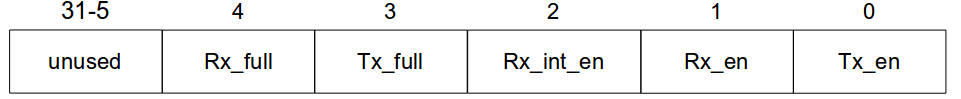
\includegraphics[width=1.0\textwidth]{./figs/serial_con_reg.png}
	\caption{Control Register}
	\label{fig2}
	\end{figure}
\subsection{Tx states}
	\begin{figure}[h!]
	\centering
	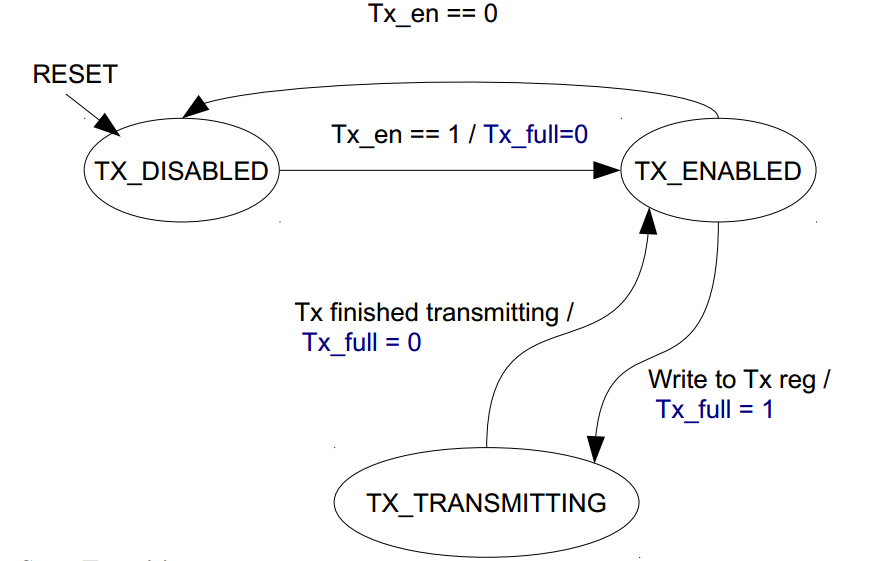
\includegraphics[width=0.9\textwidth]{./figs/tx_state.png}
	\caption{Tx state}
	\label{fig3}
	\end{figure}	
\newpage
\subsection{Rx states}
	\begin{figure}[h!]
	\centering
	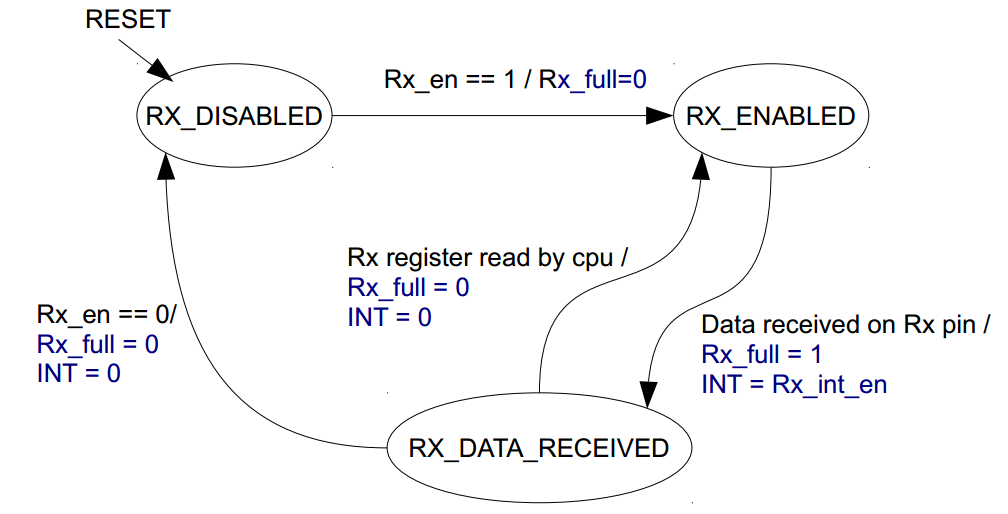
\includegraphics[width=1.0\textwidth]{./figs/rx_state.png}
	\caption{Rx state}
	\label{fig4}
	\end{figure}	
\newpage
\section{Control \& Data Flow In Ajit Serial Driver}
\subsection{Serial Driver Module Loading}
At time of module loading following functions are executed:
\begin{itemize}
\item \_\_init Ajit\_init(void).
\begin{itemize}
\item uart\_register\_driver(\&Ajit\_serial\_driver))
\item uart\_add\_one\_port(\&Ajit\_serial\_driver, \&Ajit\_port)
\item If uart\_add\_one\_port() fails then unregister serial driver by calling \\ uart\_unregister\_driver(\&Ajit\_serial\_driver)
\item end
\end{itemize}
\end{itemize} 

\subsection{Opening of Port}
\begin{itemize}
\item Ajit\_startup(struct uart\_port *port)
\begin{itemize}
\item  Request irq of no mentioned in port-\textgreater irq.\\Call Ajit\_build\_device\_irq(NULL, port-\textgreater irq).\\ If fails return error else continue.

\item call \hyperlink{requestirq}{request\_irq}(irq, Ajit\_isr, IRQF\_SHARED, AJIT\_DRIVER\_NAME, port) to request irq mentioned in port-\textgreater irq.\\ If fails return error else continue. For definition of irq please see Appendix
\item 	Ajit\_enable\_Tx(port) Enable Tx.
\item 	Ajit\_enable\_Rx(port)	Enable Rx.
\item return 0.
\end{itemize}
\item int Ajit\_request\_port(struct uart\_port *port)
\begin{itemize}
\item Request for memory to map device register in memory. it calls
 
 \textbf  {request\_mem\_region} (port-\textgreater mapbase, AJIT\_REGION, AJIT\_DRIVER\_NAME) \\
AJIT\_REGION has value of base address of control register of serial device.\\
AJIT\_REGION has size of memory to be mapped.

\item map physical address to the virtual address and store it in port-\textgreater mambase. It calls ioremap(port-\textgreater mapbase, AJIT\_REGION) \\
If port-\textgreater mambase is NULL then release memory and return -EBUSY else continue.
\item map generic platform data pointer to the private data.\\ port-\textgreater private\_data = \&Ajit\_reg\_ops 
\end{itemize}
\end{itemize}
\subsection{Transmit Char From User Space to Device}
\begin{itemize}
\item Driver calls Ajit\_start\_Tx(struct uart\_port *port). This function calls int Ajit\_Tx\_chars(struct uart\_port *port).
\item creates pointer to point TTY core's circular buffer.
\item It enables transmission by calling function Ajit\_enable\_Tx(port).
\item If port-\textgreater x\_char is true then it sends data to device, increment tx count and clears port-\textgreater x\_char. 
\item return 0 if circular buffer is empty or serial device stopped transmitting.
\item sends all 8bit data to the serial device buffer by calling function Ajit\_send\_Tx(xmit-\textgreater buf[xmit-\textgreater tail], port).\\
Here xmit-\textgreater tail points to the circular buffer of TTY core. It increment pointer by 1 at each iteration. Also it increments tx count.
\item if still there is data in TTY core circular buffer less than WAKEUP\_CHARS then it sends wakeup signal to those process which are sleeping on lock of port.
\item if circular buffer empty then sends stop signal to serial Tx.
\item return 1 as success. 
\end{itemize}
\subsection{Receive Char From Device to User Space}
\begin{itemize}
\item Serial hardware generate interrupt when it has data.
\item Receive interrupt occurs on interrupt no 12.
\item This interrupt calls Ajit\_isr(int irq, void *dev\_id).
\begin{itemize}
\item It disables all interrupt by calling Ajit\_write\_IRC\_control\_word(0x00).
\item It checks, is this interrupt generated by serial device or by any other device by calling Ajit\_receive(port). Increment value of n at each iteration.
\item It enables interrupt by calling Ajit\_write\_IRC\_control\_word(0x01).
\item if n \textgreater 1 then it returns IRQ\_HANDLED else IRQ\_NONE
\item if n \textgreater 1 it flushes receive buffer.
\end{itemize}
\end{itemize}

\subsection{Closing of Port}
\begin{itemize}
\item At time closing it first calls void Ajit\_release\_port(struct uart\_port *port). This function is  used to release memory mapped region of serial device and unmapped Virtual Address from physical address.
\item Then tty core calls Ajit\_shutdown(struct uart\_port *port) 
\begin{itemize}
\item It sends stop tx signal to serial device by using function Ajit\_stop\_Tx(port).
\item It send stop rx signal to serial device by using function Ajit\_stop\_Rx(port).
\item then it frees registered irq by calling function free\_irq(port-\textgreater irq, port).
\end{itemize}
\end{itemize}
\subsection{Serial Driver Module Unloading}
At time of module unloading following functions are executed:
\begin{itemize}
\item \_\_exit Ajit\_exit(void).
\begin{itemize}
\item uart\_unregister\_driver(\&Ajit\_serial\_driver))
\item end
\end{itemize}
\end{itemize}


\newpage
\section{Appendix}
\subsection{Linux Inbuilt Functions}
\subsubsection{ioread8}
unsigned int ioread8(void \_\_iomem *addr)\\
\_\_iomem annotation used to mark pointers to I/O memory.\\
This function is used to read 8 bit data from given memory location. Memory address is return value of ioremap().
\subsubsection{ioread32be}
unsigned int ioread32be(void \_\_iomem *addr)\\
\_\_iomem annotation used to mark pointers to I/O memory.\\
This function is used to read 32 bit data from given memory location. Memory address is return value of ioremap().
\subsubsection{iowrite8}
It is is used to write 8 bit data to device.
\subsubsection{iowrite32be}
It is is used to write 32 bit data to device.
\subsubsection{request\_irq}
\hypertarget{requestirq}{}
int \textbf{request\_irq}(unsigned int irq,
                irqreturn\_t (*handler)(int, void *, struct pt\_regs *),
                unsigned long irqflags,
                const char *devname,
                void *dev\_id)\\
This function is used to register ISR in kernel.
                      
\subsection{Definition of Function From uart\_ops }
\subsubsection{tx\_empty(port)} This function tests whether the transmitter fifo and shifter
	for the port described by 'port' is empty.  If it is empty,
	this function should return TIOCSER\_TEMT, otherwise return 0.
	If the port does not support this operation, then it should
	return TIOCSER\_TEMT. \\
Locking: none.\\
	Interrupts: caller dependent.\\
	This call must not sleep.\\
\subsubsection{set\_mctrl(port, mctrl)}
	This function sets the modem control lines for port described
	by 'port' to the state described by mctrl.  The relevant bits
	of mctrl are:\\
	
		- TIOCM\_RTS RTS signal.
		
		- TIOCM\_DTR	 DTR signal.
		
		- TIOCM\_OUT1 OUT1 signal.
		
		- TIOCM\_OUT2OUT2 signal.
		
		- TIOCM\_LOOP Set the port into loopback mode.\\ \\
	If the appropriate bit is set, the signal should be driven
	active.  If the bit is clear, the signal should be driven
	inactive.\\ 
	Locking: port-\textgreater lock taken.\\
	Interrupts: locally disabled.\\
	This call must not sleep.\\
	
\subsubsection{get\_mctrl(port)}
	Returns the current state of modem control inputs.  The state
	of the outputs should not be returned, since the core keeps
	track of their state.  The state information should include:\\
		- TIOCM\_CAR	 state of DCD signal
		
		- TIOCM\_CTS	 state of CTS signal
		
		- TIOCM\_DSR	 state of DSR signal
		
		- TIOCM\_RI	 state of RI signal\\
	The bit is set if the signal is currently driven active.  If
	the port does not support CTS, DCD or DSR, the driver should
	indicate that the signal is permanently active.  If RI is
	not available, the signal should not be indicated as active.\\ \\
	Locking: port-\textgreater lock taken.\\
	Interrupts: locally disabled.\\
	This call must not sleep.\\
\subsubsection{stop\_tx(port)} 
	Stop transmitting characters. This might be due to the CTS
	line becoming inactive or the tty layer indicating we want
	to stop transmission due to an XOFF character.
	The driver should stop transmitting characters as soon as
	possible.\\ \\
	Locking: port-\textgreater lock taken.\\
	Interrupts: locally disabled.\\
	This call must not sleep\\
\subsubsection{start\_tx(port)}
	Start transmitting characters.\\ \\
	Locking: port-\textgreater lock taken.\\
	Interrupts: locally disabled.\\
	This call must not sleep\\
\subsubsection{send\_xchar(port,ch)}
	Transmit a high priority character, even if the port is stopped.
	This is used to implement XON/XOFF flow control and tcflow().  If
	the serial driver does not implement this function, the tty core
	will append the character to the circular buffer and then call
	start\_tx() / stop\_tx() to flush the data out.\\
	Do not transmit if ch == \'\ 0\' (\_\_DISABLED\_CHAR).\\ \\
	Locking: none.\\
	Interrupts: caller dependent.\\

\subsubsection{stop\_rx(port)}
	Stop receiving characters; the port is in the process of
	being closed.\\ \\
	Locking: port-\textgreater lock taken.\\
	Interrupts: locally disabled.\\
	This call must not sleep.\\
\subsubsection{enable\_ms(port)}
	Enable the modem status interrupts.
	This method may be called multiple times. Modem status
	interrupts should be disabled when the shutdown method is
	called.\\ \\
	Locking: port-\textgreater lock taken.\\
	Interrupts: locally disabled.\\
	This call must not sleep\\

\subsubsection{break\_ctl(port,ctl)}
	Control the transmission of a break signal.  If ctl is
	nonzero, the break signal should be transmitted.  The signal
	should be terminated when another call is made with a zero
	ctl.\\ \\
	Locking: none.\\
	Interrupts: caller dependent.\\
	This call must not sleep\\

\subsubsection{startup(port)}
	Grab any interrupt resources and initialise any low level driver
	state.  Enable the port for reception.  It should not activate
	RTS nor DTR; this will be done via a separate call to set\_mctrl.
	This method will only be called when the port is initially opened.\\ \\
	Locking: port\_sem taken.\\
	Interrupts: globally disabled.\\

\subsubsection{shutdown(port)}
	Disable the port, disable any break condition that may be in
	effect, and free any interrupt resources.  It should not disable
	RTS nor DTR; this will have already been done via a separate
	call to set\_mctrl.
Drivers must not access port-\textgreater info once this call has completed.
	This method will only be called when there are no more users of
	this port.\\ \\
	Locking: port\_sem taken.\\
	Interrupts: caller dependent.\\

\subsubsection{flush\_buffer(port)}
	Flush any write buffers, reset any DMA state and stop any
	ongoing DMA transfers.
	This will be called whenever the port-\textgreater info-\textgreater  xmit circular buffer is cleared. \\ \\
	Locking: port-\textgreater lock taken.
	Interrupts: locally disabled.
	This call must not sleep

\subsubsection{set\_termios(port,termios,oldtermios)}
	Change the port parameters, including word length, parity, stop
	bits.  Update read\_status\_mask and ignore\_status\_mask to indicate
	the types of events we are interested in receiving.  Relevant
	termios-\textgreater c\_cflag bits are:\\
		CSIZE	- word size
		
		CSTOPB	- 2 stop bits
		
		PARENB	- parity enable
		
		PARODD	- odd parity (when PARENB is in force)
		
		CREAD	- enable reception of characters (if not set,
			 still receive characters from the port, but
			  throw them away.
			  
		CRTSCTS	- if set, enable CTS status change reporting
		
		CLOCAL	- if not set, enable modem status change
			  reporting.
			  
	Relevant termios-\textgreater c\_iflag bits are:
	
		INPCK	- enable frame and parity error events to be
			  passed to the TTY layer.
			  
		BRKINT
		
		PARMRK	- both of these enable break events to be
			  passed to the TTY layer.
			  
		IGNPAR	- ignore parity and framing errors
		
		IGNBRK	- ignore break errors,  If IGNPAR is also
			  set, ignore overrun errors as well.\\ \\
	The interaction of the iflag bits is as follows (parity error
	given as an example):\\ \\
\\ character received, marked as TTY\_NORMAL\\
Parity error:n/a	 INPCK:0	 IGNPAR:n/a	\\ \\
\\character received, marked as TTY\_NORMAL\\
Parity error:None INPCK:1	IGNPAR: n/a	\\ \\
character received, marked as TTY\_PARITY\\
Parity error:Yes	 INPCK:1	 IGNPAR:0\\ \\
character discarded\\
Parity error:Yes	 INPCK:1	 IGNPAR:1	\\
Other flags may be used (eg, xon/xoff characters) if your
hardware supports hardware "soft" flow control.\\ \\
Locking: caller holds port-\textgreater mutex\\
Interrupts: caller dependent.\\
This call must not sleep\\
\subsubsection{pm(port,state,oldstate)}
Perform any power management related activities on the specified
port.  State indicates the new state (defined by
enum uart\_pm\_state), oldstate indicates the previous state.
This function should not be used to grab any resources.
This will be called when the port is initially opened and finally
closed, except when the port is also the system console.  This
will occur even if CONFIG|\_PM is not set.\\ \\
Locking: none.\\
Interrupts: caller dependent.\\
\subsubsection{type(port)}
	Return a pointer to a string constant describing the specified
	port, or return NULL, in which case the string 'unknown' is
	substituted.\\ \\
	Locking: none.\\
	Interrupts: caller dependent.\\
\subsubsection{release\_port(port)}
	Release any memory and IO region resources currently in use by
	the port.\\ \\
	Locking: none.\\
	Interrupts: caller dependent.\\

\subsubsection{request\_port(port)}
	Request any memory and IO region resources required by the port.
	If any fail, no resources should be registered when this function
	returns, and it should return -EBUSY on failure.\\ \\
	Locking: none.\\
	Interrupts: caller dependent.\\
\subsubsection{config\_port(port,type)}
	Perform any autoconfiguration steps required for the port.  `type`
	contains a bit mask of the required configuration.  UART\_CONFIG\_TYPE
	indicates that the port requires detection and identification.
	port-\textgreater type should be set to the type found, or PORT\_UNKNOWN if no port was detected.\\

	UART\_CONFIG\_IRQ indicates auto-configuration of the interrupt signal,
	which should be probed using standard kernel auto-probing techniques.
	This is not necessary on platforms where ports have interrupts
	internally hard wired (eg, system on a chip implementations).\\ \\
	Locking: none.\\
	Interrupts: caller dependent.\\

\subsubsection{verify\_port(port,serinfo)}
	Verify the new serial port information contained within serinfo is
	suitable for this port type.\\ \\
	Locking: none.\\
	Interrupts: caller dependent.\\

\subsubsection{ioctl(port,cmd,arg)}
	Perform any port specific IOCTLs.  IOCTL commands must be defined
	using the standard numbering system found in \textless asm/ioctl.h \textgreater \\ \\
	Locking: none.\\
	Interrupts: caller dependent.\\

\subsubsection{poll\_init(port)}
	Called by kgdb to perform the minimal hardware initialization needed
	to support poll\_put\_char() and poll\_get\_char().  Unlike -\textgreater startup() this should not request interrupts.\\ \\
	Locking: tty\_mutex and tty\_port-\textgreater mutex taken.\\
	Interrupts: n/a.\\

\subsubsection{poll\_put\_char(port,ch)}
	Called by kgdb to write a single character directly to the serial
	port.  It can and should block until there is space in the TX FIFO.\\ \\
	Locking: none.\\
	Interrupts: caller dependent.\\
	This call must not sleep\\
\subsubsection{poll\_get\_char(port)}
	Called by kgdb to read a single character directly from the serial
	port.  If data is available, it should be returned; otherwise
	the function should return NO\_POLL\_CHAR immediately.\\ \\
	Locking: none.\\
	Interrupts: caller dependent.\\
	This call must not sleep.	\\ \\

\end{document}
